% Videos: steganography, LSB steganography demo, cryptography solved questions, abstract algebra & number theory intro, prime numbers
\definecolor{puregreen}{RGB}{0,255,0}
\definecolor{modgreen}{RGB}{0,252,0}

\section{Steganography}

\begin{keybox}
\textbf{Steganography} \textbf{conceals the existence} of the message: the message is hidden. It is \textbf{not an encryption scheme}.\\
\textbf{Cryptography} renders the message \textbf{unintelligible} to outsiders by transforming the text.
\end{keybox}
\begin{center}\small
\begin{tabularx}{\textwidth}{@{}l X X@{}}
\toprule
 & \textbf{Cryptography} & \textbf{Steganography}\\
\midrule
Hides & the \textbf{meaning} & the \textbf{existence}\\
Attacker sees & a scrambled message; knows something secret is being sent & an ordinary-looking text/image; doesn't suspect anything\\
Output & ciphertext & a normal-looking \textbf{cover} (text, image, audio) with the message inside\\
\bottomrule
\end{tabularx}
\end{center}
This is the other kind of ``security-related transformation $T$'' mentioned in the network security model (Section 1): $T$ doesn't have to be encryption.

\textbf{Examples from the lecture} (read the first letters):
\begin{itemize}
  \item \textbf{S}imply \textbf{e}ncrypt \textbf{c}orrect \textbf{r}eading \textbf{e}xactly \textbf{t}wice. $\Rightarrow$ \textbf{Secret}
  \item \textbf{T}ell \textbf{h}enry \textbf{a}lice \textbf{n}ot \textbf{k}ane / \textbf{Y}esterday \textbf{o}urplan \textbf{u}ndone! $\Rightarrow$ \textbf{Thank You}
\end{itemize}

\subsection{Historical techniques}
\begin{center}\small
\begin{tabularx}{\textwidth}{@{}l X@{}}
\toprule
Character marking & Chosen letters of a printed text are overwritten faintly in pencil. Visible only when the paper is held at an angle to bright light.\\
Invisible ink & Written with a substance (e.g.\ lemon juice) that leaves no trace until heat or a chemical is applied.\\
Pin punctures & Tiny pin holes on selected letters. Invisible until the paper is held up to a light.\\
Typewriter correction ribbon & Text typed between the lines with a correction ribbon. Visible only under strong light.\\
\bottomrule
\end{tabularx}
\end{center}

\subsection{Drawbacks}
\begin{enumerate}[leftmargin=1.5em]
  \item \textbf{Lots of overhead}: a large cover is needed to hide a few bits of message.
  \item \textbf{Once the system is discovered, it becomes virtually worthless}. Unlike encryption, there is no secret key left to protect the message.
\end{enumerate}
\begin{keybox}[title=Best of both]
A message can be \textbf{first encrypted and then hidden} using steganography. If the hiding is discovered, the attacker still only has ciphertext.
\end{keybox}
\begin{center}
\begin{tikzpicture}[node distance=6mm]
  \node[box,fill=cyan!10] (p) {Plaintext};
  \node[box,fill=green!15,right=of p] (e) {Encrypt\\(key)};
  \node[box,fill=yellow!20,right=of e] (c) {Ciphertext};
  \node[box,fill=orange!15,right=of c] (h) {Hide in\\cover};
  \node[box,fill=gray!15,above=4mm of h] (cv) {Cover image};
  \node[box,fill=magenta!8,right=of h] (s) {Stego image\\(looks normal)};
  \draw[arr] (p)--(e); \draw[arr] (e)--(c); \draw[arr] (c)--(h); \draw[arr] (cv)--(h); \draw[arr] (h)--(s);
\end{tikzpicture}
\end{center}

\subsection{LSB steganography}
\textbf{LSB} = least significant bit(s): the rightmost bits of a number, which change its value the least.
\[
1010\,10\underbrace{01}_{\text{LSBs}} \qquad\text{bit weights: } 128\;64\;32\;16\;8\;4\;\underline{2\;1}
\]
\textbf{RGB model:} each pixel is 24 bits, 8 each for Red, Green and Blue (0--255).
\begin{center}\small Red $(255,0,0) = (\ttx{11111111}, \ttx{00000000}, \ttx{00000000})$ \quad Green $(0,255,0)$ \quad Blue $(0,0,255)$\end{center}

\begin{center}
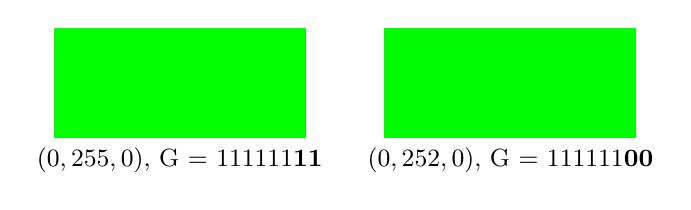
\begin{tikzpicture}
  \fill[puregreen] (0,0) rectangle (3.2,1.4);
  \fill[modgreen] (4.2,0) rectangle (7.4,1.4);
  \node[font=\small,below] at (1.6,0) {$(0, 255, 0)$, G $=$ \ttx{111111\textbf{11}}};
  \node[font=\small,below] at (5.8,0) {$(0, 252, 0)$, G $=$ \ttx{111111\textbf{00}}};
\end{tikzpicture}
\end{center}
The two boxes look identical, but the last 2 bits differ. \textbf{Those LSBs can store hidden information.}
Using 2 LSBs in each of R, G and B hides $2 \times 3 = \mathbf{6}$ \textbf{bits per pixel}, and no channel value changes by more than 3.

\textbf{Worked example} (mine): hide the bits \ttx{11 01 10} in the pixel $(100, 50, 200)$:
\begin{center}\small
\begin{tabular}{@{}lllll@{}}
\toprule
Channel & Value & Binary & Replace last 2 bits & New value\\
\midrule
R & 100 & \ttx{011001\textbf{00}} & \ttx{011001\textbf{11}} & 103 ($+3$)\\
G & 50 & \ttx{001100\textbf{10}} & \ttx{001100\textbf{01}} & 49 ($-1$)\\
B & 200 & \ttx{110010\textbf{00}} & \ttx{110010\textbf{10}} & 202 ($+2$)\\
\bottomrule
\end{tabular}
\end{center}
To extract, the receiver just reads the last 2 bits of each channel. \textbf{Capacity:} an $800\times600$ image holds $800 \cdot 600 \cdot 6 = 2{,}880{,}000$ bits $= 360{,}000$ bytes.

\textbf{Blue orchids:} the lecture shows the image without and with hidden information side by side, and you can't tell them apart.

\subsection{Watermarking vs.\ image steganography}
\begin{center}\small
\begin{tabularx}{\textwidth}{@{}l X X@{}}
\toprule
 & \textbf{Watermarking} & \textbf{Image steganography}\\
\midrule
Purpose & prove \textbf{ownership} / copyright & \textbf{secret communication}\\
Is the mark secret? & no; it's often visible (like the \ttx{nesoacademy.org} logo) & yes; its \textbf{existence} is hidden\\
Hidden data & logo, owner info & any message or file\\
\bottomrule
\end{tabularx}
\end{center}

\subsection{OpenStego demo}
\begin{enumerate}[leftmargin=1.5em]
  \item \textbf{Hide Data:} message file \ttx{My Message.txt} (``Kill Corona Virus'', 17 bytes) + cover file \ttx{Blue Orchids.jpg} (58.4 KB) $\to$ stego file \ttx{BO.png} (824 KB). No password. ``Message embedded into 1 cover file(s).''
  \item \textbf{Extract Data:} input \ttx{BO.png} $\to$ output folder. ``Message file extracted successfully'', and the text file comes back unchanged.
\end{enumerate}
{\small\emph{Why PNG and why so much bigger (not explained in the video):} JPEG compression slightly changes pixel values, which would wipe out the LSBs. So the stego image is saved in the lossless PNG format, which is much larger. That size jump is itself a hint something is going on.}

\section{Solved Exam Questions}

\textbf{Q1.} Sender and receiver use the \textbf{same key}: \textbf{(b) private key} and \textbf{(c) symmetric} cryptography are both correct (two names for the same thing).

\textbf{Q2.} $19 \bmod 3$: $19 = 6 \cdot 3 + \mathbf{1}$, so the answer is \textbf{(d) 1}. (mod gives the remainder.)

\textbf{Q3 (UGC NET 2016).} An attacker captures information and \textbf{retransmits it later without altering it}. Options: DoS / masquerade / simple / complex. Official answer: \textbf{(a) denial of service}. Reason given: repeated retransmissions flood the receiver so it can't serve real users.
\begin{keybox}[title=Exam note]
The textbook name for ``capture and retransmit later'' is a \textbf{replay attack}. If \emph{replay} is one of the options, choose it. Here it isn't, so DoS is the best available answer.
\end{keybox}

\textbf{Q4 (ISRO 2020).} Columnar transposition, plaintext ``the tomato is a plant in the night shade family'', keyword \textbf{TOMATO}.
38 letters, 6 columns $\Rightarrow$ 7 rows (42 cells), 4 fillers \ttx{x}. Number the keyword letters alphabetically; \textbf{for repeated letters, go left to right}:
\begin{center}\small
\begin{minipage}[c]{0.4\textwidth}\centering
\begin{tabular}{|*{6}{c|}}
\multicolumn{1}{c}{T}&\multicolumn{1}{c}{O}&\multicolumn{1}{c}{M}&\multicolumn{1}{c}{A}&\multicolumn{1}{c}{T}&\multicolumn{1}{c}{O}\\
\multicolumn{1}{c}{5}&\multicolumn{1}{c}{3}&\multicolumn{1}{c}{2}&\multicolumn{1}{c}{\textbf{1}}&\multicolumn{1}{c}{6}&\multicolumn{1}{c}{4}\\
\hline
t&h&e&\cellcolor{warn!18}t&o&m\\\hline
a&t&o&\cellcolor{warn!18}i&s&a\\\hline
p&l&a&\cellcolor{warn!18}n&t&i\\\hline
n&t&h&\cellcolor{warn!18}e&n&i\\\hline
g&h&t&\cellcolor{warn!18}s&h&a\\\hline
d&e&f&\cellcolor{warn!18}a&m&i\\\hline
l&y&\textit{x}&\cellcolor{warn!18}\textit{x}&\textit{x}&\textit{x}\\\hline
\end{tabular}
\end{minipage}
\begin{minipage}[c]{0.5\textwidth}
Read order A, M, O, O, T, T $=$ columns 4, 3, 2, 6, 1, 5:\\[3pt]
\ttx{TINESAX EOAHTFX HTLTHEY MAIIAIX TAPNGDL OSTNHMX}\\[3pt]
Answer: \textbf{(a)}.\\[2pt]
{\footnotesize (The slide gave both O's the number 3 and both T's the number 4, then read left to right. That is the same order.)}
\end{minipage}
\end{center}

\textbf{Q5 (GATE 2015).} $N$ people, every pair needs its own \textbf{symmetric} key that nobody else knows. One key per pair:
\[
\binom{N}{2} = \frac{N(N-1)}{2} \qquad (N=2: 1,\; N=3: 3,\; N=4: 6,\; N=5: 10) \qquad\text{Answer: \textbf{(c)}}
\]
{\small\emph{Common follow-up (not in the video):} with \textbf{public-key} cryptography, each person needs just one key pair: $N$ pairs, $2N$ keys in total. This is one big reason public-key cryptography exists.}

\section{Prime Numbers}
\begin{keybox}
\textbf{Prime}: $> 1$ with exactly two divisors (1 and itself). \textbf{Composite}: more than two divisors. \textbf{1 is neither}; 2 is the only even prime. Every $n > 1$ factors uniquely into primes (fundamental theorem of arithmetic), e.g.\ $14688 = 2^5 \cdot 3^3 \cdot 17$.
\end{keybox}
\subsection{Why primes matter in cryptography}
\begin{keybox}
Many encryption algorithms (e.g.\ RSA) are based on primes. \textbf{Multiplying} two large primes is \textbf{very fast}. The \textbf{reverse} (\textbf{factoring} the product back into its primes) is \textbf{extremely slow}.
\end{keybox}
\[
p, q \;\xrightarrow{\text{easy}}\; n = p \cdot q \qquad\qquad n \;\xrightarrow{\text{very hard}}\; p, q
\]
This ``easy one way, hard to reverse'' shape is called a \textbf{one-way (trapdoor) function}.


\begin{examtip}
\begin{itemize}
  \item Steganography hides the \emph{existence}; cryptography hides the \emph{meaning}. Steganography is not encryption.
  \item Two drawbacks: lots of overhead; worthless once discovered. Fix: encrypt first, then hide.
  \item LSB: 2 LSBs $\times$ 3 channels $=$ 6 bits per pixel; each value changes by at most 3.
  \item Watermarking proves ownership (not secret); steganography hides communication.
  \item Symmetric keys for $N$ people: $N(N-1)/2$. Public key: $N$ pairs.
  \item Columnar key with repeated letters: number them left to right.
  \item 1 is not prime; 2 is the only even prime. Security rests on \emph{factoring the product} being hard.
\end{itemize}
\end{examtip}

\begin{fixbox}
\begin{itemize}
  \item \textbf{Slide wording:} ``Factoring very large prime numbers is very hard'' should say factoring the \emph{product} of two large primes. A prime can't be factored at all.
  \item The factorisation table writes $11 = 1^1 \times 11^1$ and lists 1 as a prime factor. 1 is not prime; 11 and 37 are simply prime.
  \item The notes call watermarks ``typically visible''. The lecture's example is visible, but watermarks can also be invisible. The real difference is the purpose (ownership vs.\ secret communication).
  \item Fermat's and Euler's theorems need $\gcd(a,p) = 1$ / $\gcd(a,n) = 1$; the notes omitted this condition.
  \item Everything else checked: TOMATO $\to$ (a) (by script), $N(N-1)/2$, all six numbers prime, factorisations correct.
\end{itemize}
\end{fixbox}
